%%%%%%%%%%%%%%%%%%%%%%%%%%%%%%%%%%%%%%%%%%%%%%%%%%%%%%%%%%%%%%%%%%%%%%%%
%                                                                      %
%     File: Thesis_Introduction.tex                                    %
%     Tex Master: Thesis.tex                                           %
%                                                                      %
%     Author: Andre C. Marta                                           %
%     Last modified :  05 Aug 2026                                     %
%                                                                      %
%%%%%%%%%%%%%%%%%%%%%%%%%%%%%%%%%%%%%%%%%%%%%%%%%%%%%%%%%%%%%%%%%%%%%%%%

\chapter{Introduction}
\label{chapter:introduction}

This chapter introduces the thesis, presenting the context, motivation, and objectives of the research, followed by an overview of the system architecture, the expected scientific and engineering contributions, and the overall structure of the dissertation.

\section{Motivation}
\label{sec:intro_motivation}

Saving lives at sea, protecting marine ecosystems, and securing maritime infrastructure all rely on one essential capability: understanding what is happening, where, and when. In vast and dynamic maritime environments, this requires maintaining reliable, high-resolution situational awareness over long periods. The \gls{emsa} recognises this challenge and highlights the need for continuous monitoring and locally persistent operations to enable effective maritime surveillance and response~\cite{europeanmaritimesafetyagencyEMSAOutlook2025_v302025}.

Different maritime assets meet this challenge in complementary ways. Surface vessels give a physical presence at sea, with long endurance and large payload capacity~\cite{introduction_motivation_vessel_sensors,introduction_motivation_vessel_tasks}. However, their range is limited by line of sight, and operations are expensive~\cite{introduction_motivation_vessel_limitations}. Aerial platforms, such as manned aircraft and \glspl{uav}, allow fast deployment and elevated sensing~\cite{introduction_motivation_aerial_surveillance}. Yet, aircraft are costly, and \glspl{uav} suffer from low endurance and unreliable communication~\cite{introduction_motivation_uavs_limitations}.

Together, these assets form a connected system rather than separate solutions. Each one compensates for what the other lacks. \glspl{usv} provide long-term presence at sea at much lower cost than crewed vessels, allowing wide and affordable patrols. \glspl{uav} extend this reach by sensing beyond the horizon from the air. Working as a team, they maintain continuous and local maritime awareness. This motivates the study of coordinated \gls{usv}--\gls{uav} systems, where cooperation creates mission capabilities that neither platform can achieve alone in complex and changing environments.

A natural way to strengthen this cooperation is to add a physical tether between both platforms. The tether provides continuous power and reliable communication between the \gls{usv} and \gls{uav}~\cite{introduction_motivation_tethered_drones}. By placing the energy supply and communication systems on the \gls{usv}, it overcomes two main limits of maritime \glspl{uav}: short endurance and weak long-range communication. This approach has recently transitioned from academic concepts to real-world industrial systems; for instance, the marine robotics company Exail partnered with Elistair to integrate a tethered quadrotor directly onto the DriX USV catamaran for persistent maritime surveillance~\cite{exail_elistair_tethered}. Similarly, ACUA Ocean and Teledyne FLIR Defense demonstrated an integrated tethered aerial-surface system for the UK Ministry of Defence to support long-endurance maritime security and target detection~\cite{acua_ocean_teledyne_mod}.

Figure~\ref{fig:tether_scheme} illustrates the configuration of the tethered \gls{usv}--\gls{uav} system considered in this work.

\begin{figure}[H]
    \centering
    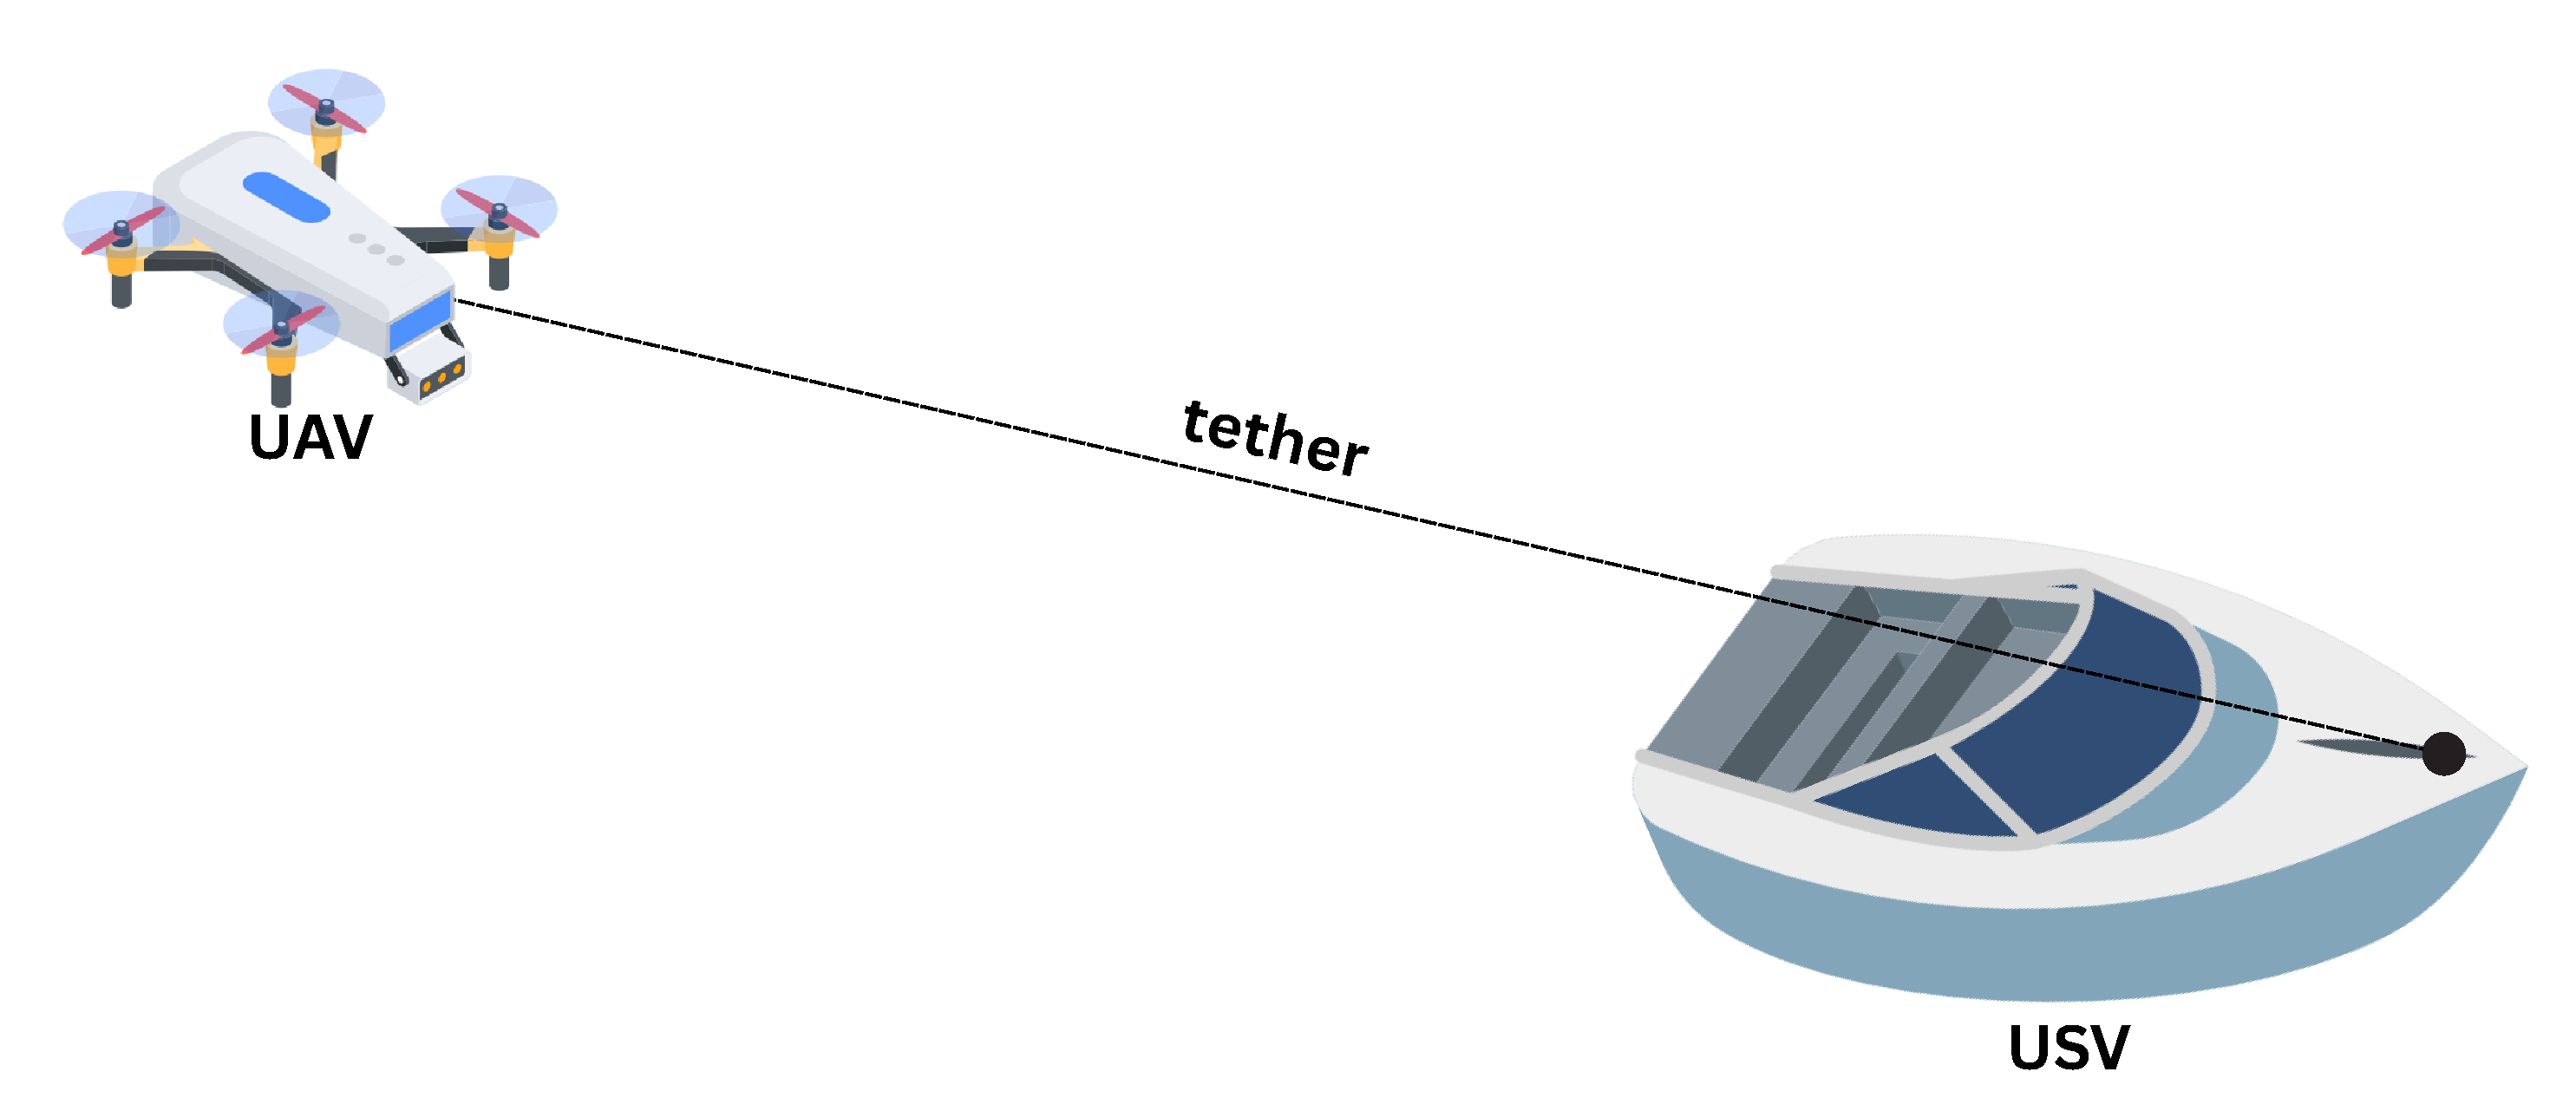
\includegraphics[width=0.65\linewidth]{Figures/introduction/system.pdf}
    \caption{Schematic of a tethered \gls{usv}--\gls{uav} system.}
    \label{fig:tether_scheme}
\end{figure}

The main challenge of this work is to design a control framework that enables two autonomous vehicles, connected by a tether, to operate as a single coordinated system. The controller must manage not only the motion of both vehicles but also account for the tether constraints and dynamics, ensuring safe operation and robustness to wind, waves, and obstacles.

The \gls{usv} and \gls{uav} operate under very different dynamics. The \gls{usv} moves slowly, dominated by hydrodynamic drag and inertia, while the \gls{uav} reacts quickly, with motion evolving on much shorter time scales. Coordinated control is challenging because the controller must handle these different response rates and actuation dynamics consistently.

The maritime environment adds further complexity. Wind, waves, and water motion constantly disturb both platforms, making robustness to disturbances essential. Nearby structures, vessels, or obstacles can restrict their movement and risk tether entanglement. Effective cooperation relies on continuous information exchange and synchronised decision-making between both agents.

Most existing tethered \gls{uav} systems focus on power delivery and communication, with operation often remaining manual or semi-autonomous. In research prototypes, the aerial and surface vehicles are usually decoupled, the tether is simplified or linearised, or the surface platform is treated as fixed. These assumptions make control design easier but reduce realism. Few cooperative control approaches explicitly model the tether while coordinating both agents under realistic maritime conditions.

\section{Problem Statement}
\label{sec:intro_problem_statement}

This work addresses the problem of controlling a cooperative system composed of an autonomous surface vessel (the WAM-V USV) and a physically connected quadrotor (the x500 UAV) operating in a coordinated manner. The objective of such a system is to autonomously execute maritime missions by following predefined waypoints or continuous reference trajectories, while respecting the physical and operational constraints of both platforms and of the tether that connects them.

To achieve this objective, the control framework must be capable of handling different phases of operation and mission requirements. This includes the definition of multiple control modes that allow the system to perform manoeuvres such as takeoff and landing, as well as different forms of coordinated motion during navigation. The UAV NMPC must actively prevent the tether from exceeding its maximum physical length, utilizing soft constraints and slacks, while the USV NMPC coordinates the planar movement of the dynamic anchor deck.

\section{System Overview}
\label{sec:intro_system_overview}

Interaction with the system is defined at the mission level. The operator selects a mission, such as patrolling a given area, following a moving target, or visiting a set of waypoints that represent regions of interest. This mission information is received by a behaviour management layer, which selects the active control mode and handles mission logic, including switching between different relative configurations of the \gls{uav} with respect to the \gls{usv}, as well as executing specific manoeuvres such as takeoff and landing.

Based on the selected mission and active control mode, the system generates coordinated motion for both the \gls{usv} and the \gls{uav}. This process combines planning and control to compute trajectories and actuation commands that satisfy vehicle and tether constraints while pursuing the mission objectives. The WAM-V USV acts as the leader planar platform carrying an active winch system on its deck. The winch dynamically spools the tether in or out to manage slack and cable tension. The x500 UAV follows a relative orbit or observation trajectory above the USV, using its elevated perspective to record visual data.

Figure~\ref{fig:placeholder} presents a high-level block diagram of the proposed system, showing the interaction between the coordinator, the decentralized NMPC solvers, the vehicles, and the co-simulation interfaces.

\begin{figure}[H]
    \centering
    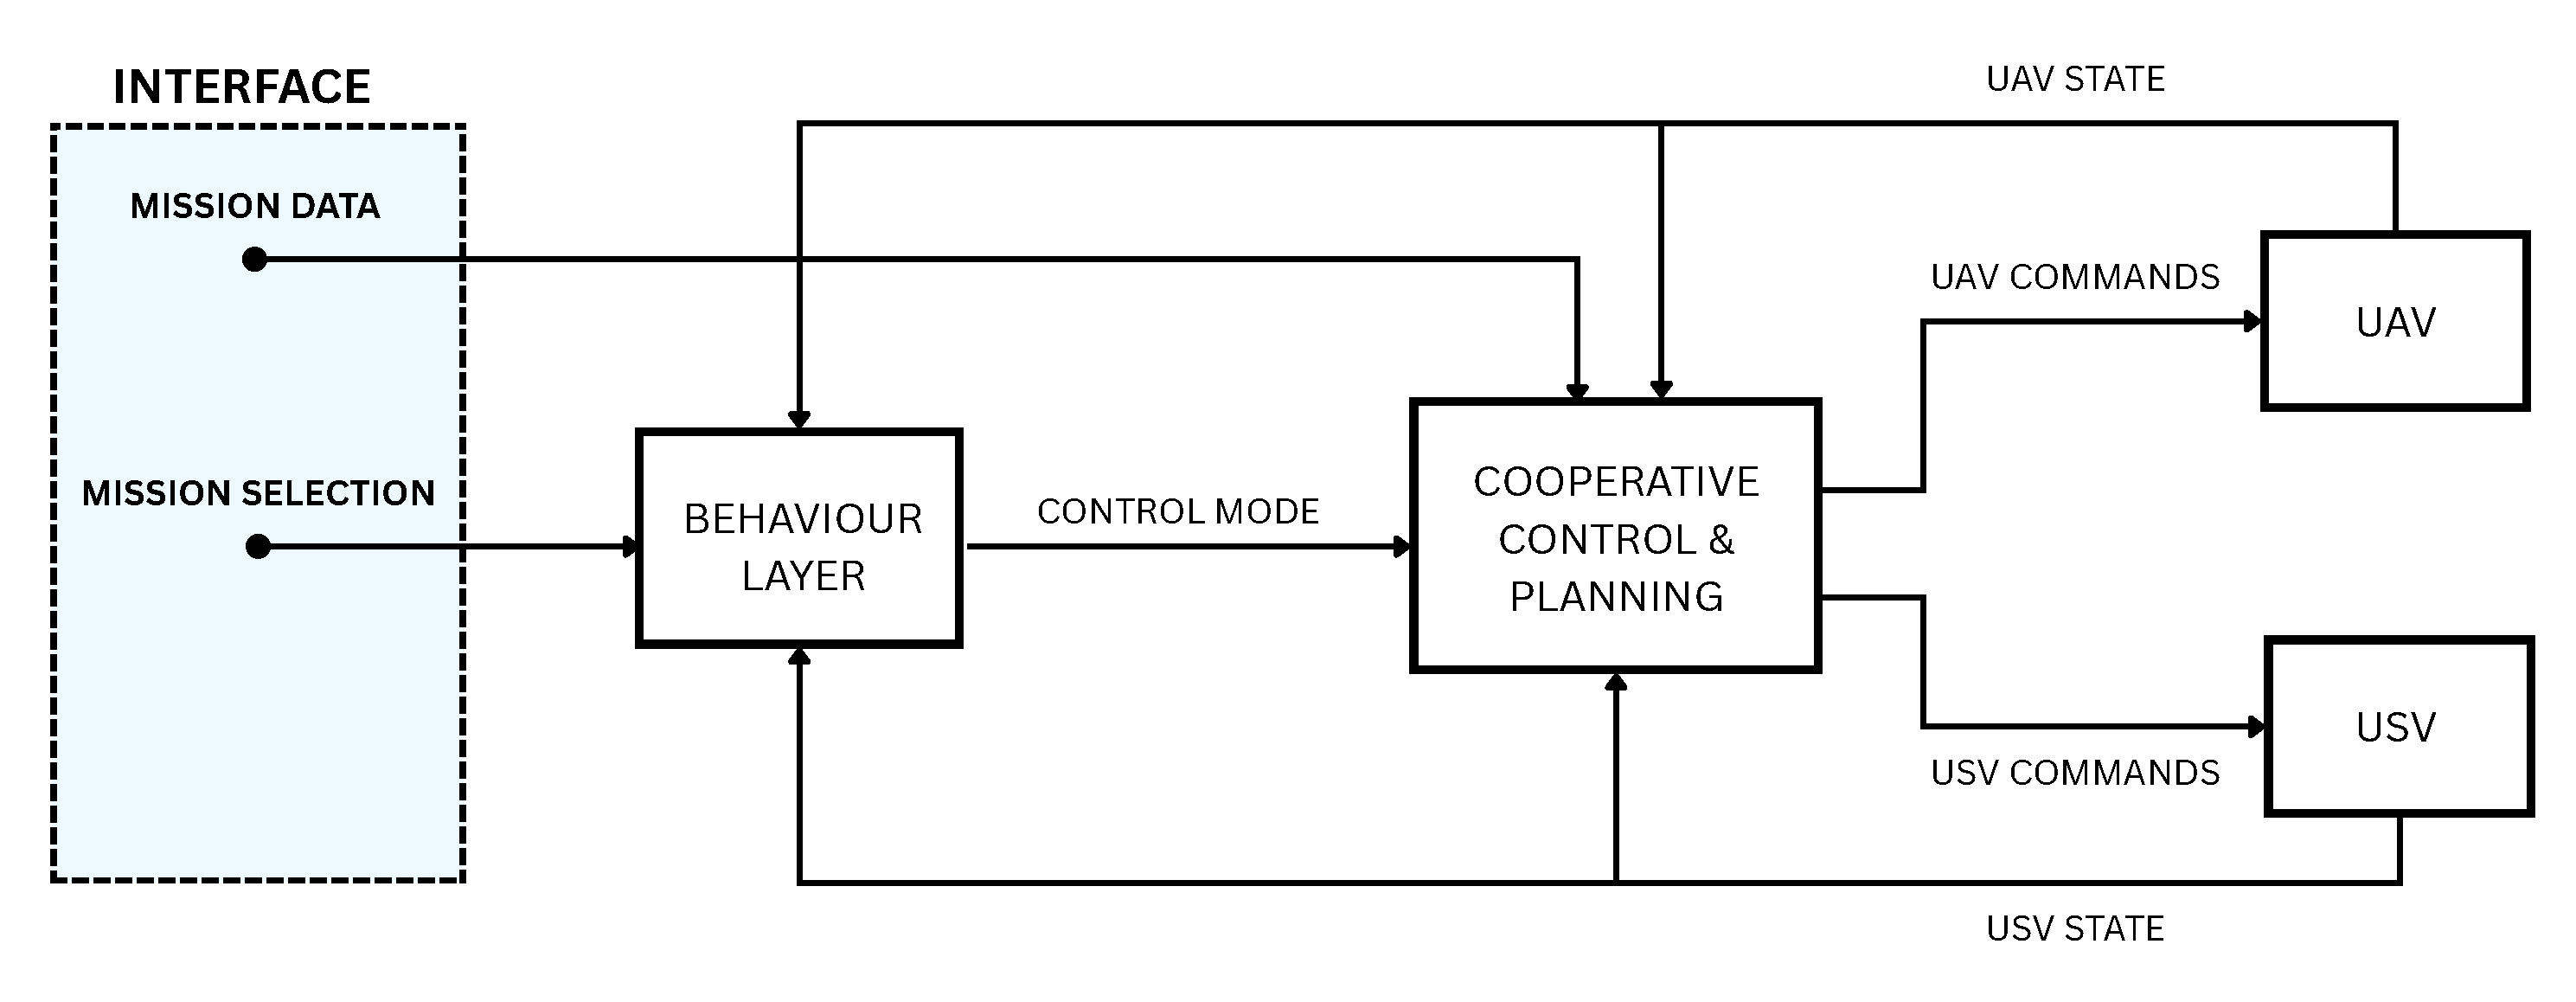
\includegraphics[width=0.85\linewidth]{Figures/introduction/block_diagram.pdf}
    \caption{High-level block diagram of the proposed cooperative control system.}
    \label{fig:placeholder}
\end{figure}

\section{Expected Contributions}
\label{sec:intro_contributions}

This thesis contributes to the design, implementation, and evaluation of cooperative control solutions for tethered \gls{uav}--\gls{usv} systems, to enable autonomous and persistent maritime missions. The main contributions of this work are summarised as follows:

\begin{itemize}
    \item A unified, C++ ROS 2 control pipeline utilizing Acados and HPIPM to generate and execute real-time Nonlinear Model Predictive Control solvers for both surface tracking and aerial guidance.
    \item The modeling and experimental identification of the UAV inner-loop attitude response lag ($\tau = 0.15\,\text{s}$) using PX4 doublets flight data.
    \item The design and implementation of a virtual winch controller operating in both geometric and tension-feedback PD modes to prevent cable slackness and tension spikes.
    \item A realistic co-simulation setup in Gazebo Harmonic, integrated with the PX4 Software-in-the-Loop (SITL) firmware and the MoorDyn physics engine for multi-body lumped-mass line representation.
    \item The verification of NMPC constraints enforcement (states, inputs, and tether length limits) and evaluation of solver latency.
    \item The validation of the entire cooperative control stack under an integrated search and pursuit mission targeting a vessel teleoperated in real-time.
\end{itemize}

\section{Thesis Structure}
\label{sec:intro_structure}

The remainder of this dissertation is organized as follows:
\begin{itemize}
    \item \textbf{Chapter 2 (Literature Review and State of the Art)} reviews existing research in cooperative marine-aerial robotics, tethered drones, and predictive control algorithms.
    \item \textbf{Chapter 3 (Virtual Platforms and Simulation Setup)} introduces the physical characteristics of the WAM-V catamaran, the x500 quadrotor, and the Gazebo simulation environment parameters.
    \item \textbf{Chapter 4 (System Modeling and Validation)} derives the kinematic and dynamic models of both vehicles, validates the UAV attitude response, and models the physical tether and winch equations.
    \item \textbf{Chapter 5 (Cooperative Control Design)} details the decentralized NMPC mathematical formulation, cost functions, physical constraints, and winch spooling control laws.
    \item \textbf{Chapter 6 (Implementation)} explains the modular ROS 2 workspace, the Library + Wrapper design pattern in C++, the mission state machine, and the communication bridges.
    \item \textbf{Chapter 7 (Results and Discussion)} evaluates tracking precision, constraint enforcement, solver latency, and the target interception mission.
    \item \textbf{Chapter 8 (Conclusions and Future Work)} summarizes the findings of the thesis and outlines directions for future research.
\end{itemize}
